\documentclass[a4paper,12pt]{article}
\usepackage{graphicx}
\usepackage{float}
\usepackage{hyperref}
\usepackage{subcaption}
\graphicspath{ {./images/} }

%opening
\title{Warsaw scanning report}
\author{Miłosz Wojciechowski}
\date{\today}

\begin{document}


\maketitle
\pagebreak
\tableofcontents
\pagebreak

\section{Introduction}
This document serves as a report for Mandeye dev (documentation available \href{link}{here}) scanning process of Warsaw city. For every scan its planned route, covered route and date will be provided. Scans were performed using Mandeye mobile scanning system. Routes were planned and visualized in QGIS (podaj link do qgisa) using database BDOT10k (podaj link do bdota) and covered routes where registered by a GoPro MAX camera and its GNSS. File structure: Folder with scanning results and with folder containing GoPro recordings. GoPro recording means 3 files: .360, .LRV and THM file but only .360 and .LRV files are used in the project.

\section{Week 11-15 September 2023}
It was a week with first scans and served as a test of how should it be done. Two scans were conducted - on Wednesday and Thursday. 
\begin{enumerate}
	\item \textbf{13.09.2023} Wednesday scan focused on Palace of Culture and Science and its surroundings and was supposed to achieve 10km of covered track. It was a pure test of the hardware thus no plan was prepared although the planned route (Fig.1a) was estimated to be 6.97km after the scan had been conducted (based on covered route). The covered route (Fig.1b) was equal to 7,12km and took 1 hour 16 minutes. Purpose of this scan was to observe how the scanner is handling city buildings as well as to try a 360 video camera mode. Unfortunately camera battery ran low and the scan had to be ended before getting to desired 10km. Moreover this test revealed a tremendous problem with the GPS localization of the GoPro camera as can be seen below. This is also the only scan that used smartwatch Huawei Watch GT as a basis for determining the covered route length, since the GPS record from GoPro was subject to vast error.
	\begin{figure}[H]
		\centering
		\begin{subfigure}{.90\textwidth}
			\centering
			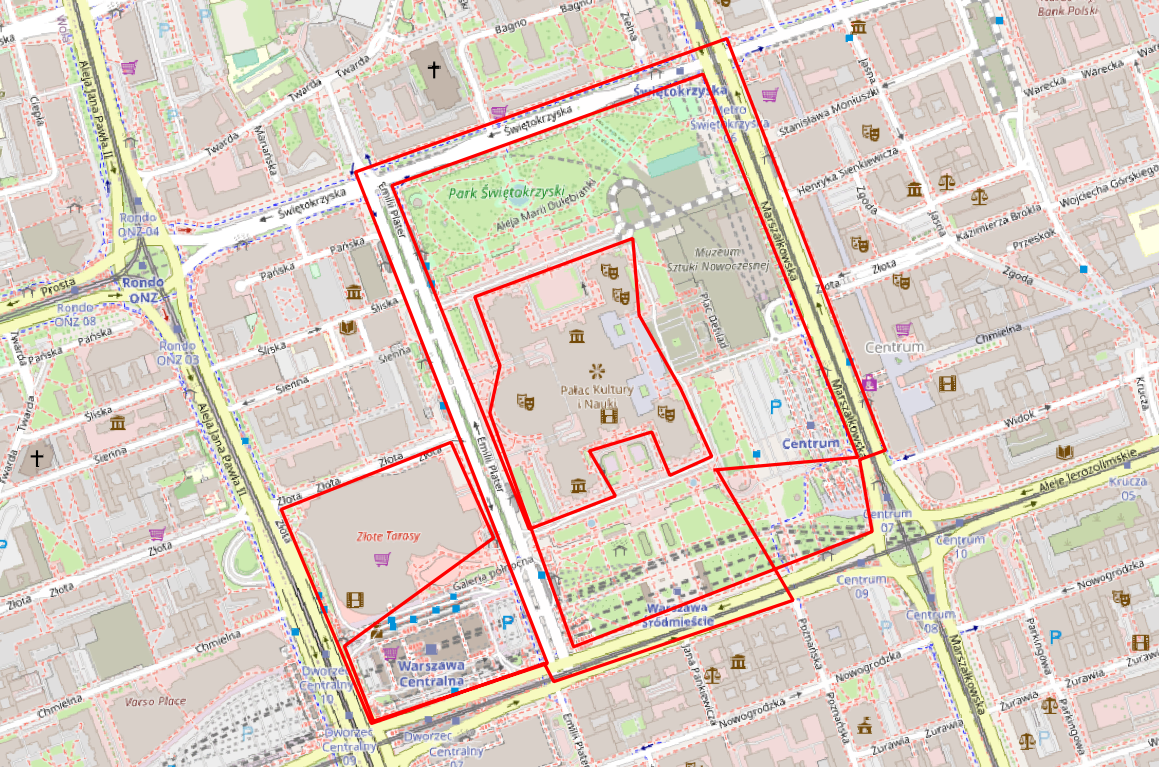
\includegraphics[width=1\linewidth]{route_p0}
			\caption{Planned route}
			\label{fig:a0}
		\end{subfigure}%
		\linebreak
		\begin{subfigure}{.90\textwidth}
			\centering
			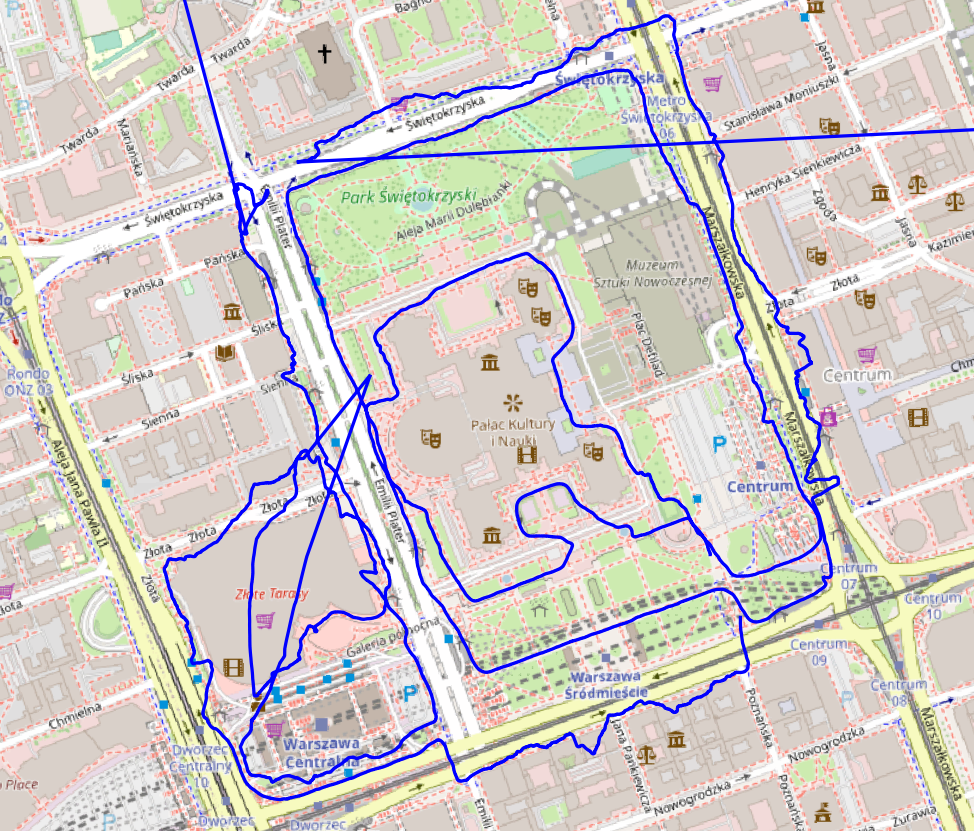
\includegraphics[width=1\linewidth]{route_c0}
			\caption{Covered route}
			\label{fig:b0}
		\end{subfigure}
		\caption{Planned and covered routes.}
		\label{fig:fig0}
	\end{figure}	
	\item \textbf{14.09.2023} Second scan on Thursday was the one to test second 360 recording mode - Time Lapse. It performed significantly better than normal video as the battery went down to roughly \verb|40%| and localization proved to be more precise without such enormous errors. With prolonged battery working time I could achieve almost 10km distance (more precisely 9,64km (Fig. 3b)) of the planned 9,46 (Fig. 3a). However such long routes proved to be too exhausting to be conducted every day for the next 2 months and thus daily track length was lowered to approximately 5km. After this scan, Friday was a day to rest, since I couldn't perform any more scans due to fatigue. 
	\begin{figure}[H]
		\centering
		\begin{subfigure}{.88\textwidth}
			\centering
			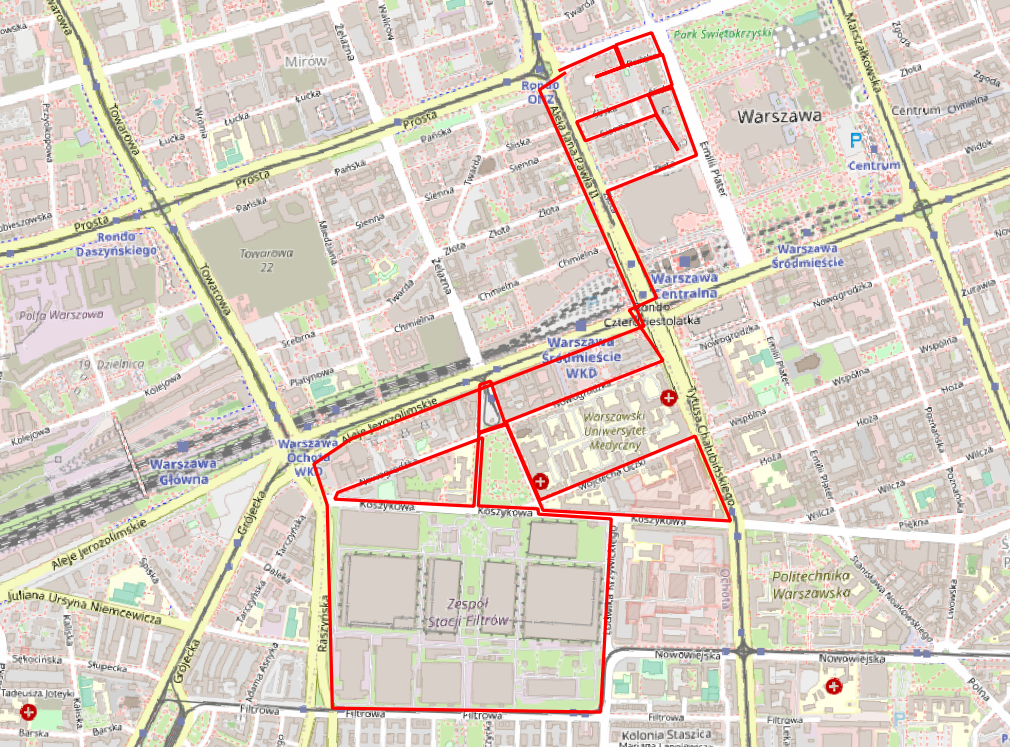
\includegraphics[width=1\linewidth]{route_p1}
			\caption{Planned route}
			\label{fig:a1}
		\end{subfigure}%
		\linebreak
		\begin{subfigure}{.88\textwidth}
			\centering
			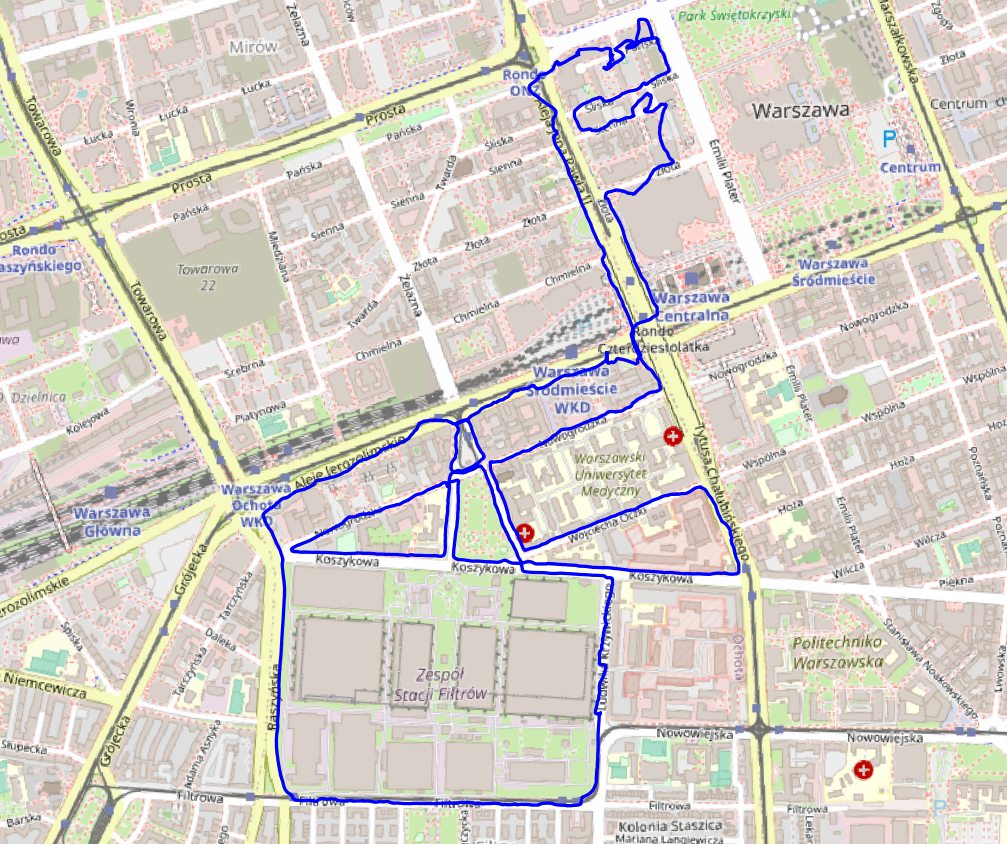
\includegraphics[width=1\linewidth]{route_c1}
			\caption{Covered route}
			\label{fig:b1}
		\end{subfigure}
		\caption{Planned and covered routes.}
		\label{fig:fig1}
	\end{figure}
\end{enumerate}
A vital conclusion after the first test scans is that Time Lapse mode should be utilized for scanning purposes due to its higher GPS accuracy and lower battery usage resulting in longer and more precise scans.
\section{Week 18-22 September 2023}
It was a week for first fully planned scans, with complete setup. 
\begin{enumerate}
	\item \textbf{18.09.2023} On Monday, after the weekend rest, I conducted the first scan. It included all streets in an area beetwen Jerozolimskie avenue, Prosta street, Zelazna street and Jana Pawla II avenue. The planned route (Fig. 3a) was estimated to be 6,48km but the covered route (Fig. 3b) ended up to be a little bit higher - 6,59km which took 1 hour 21 minutes. The difference was caused by the need to scan a parking lot and an alley next to a skyscraper located between Chmielna street and Jerozolimskie avenue and probably because, as seen in the figure 3b, there appeared to be a localization problems in smartwach software.
	\begin{figure}[H]
		\centering
		\begin{subfigure}{.90\textwidth}
			\centering
			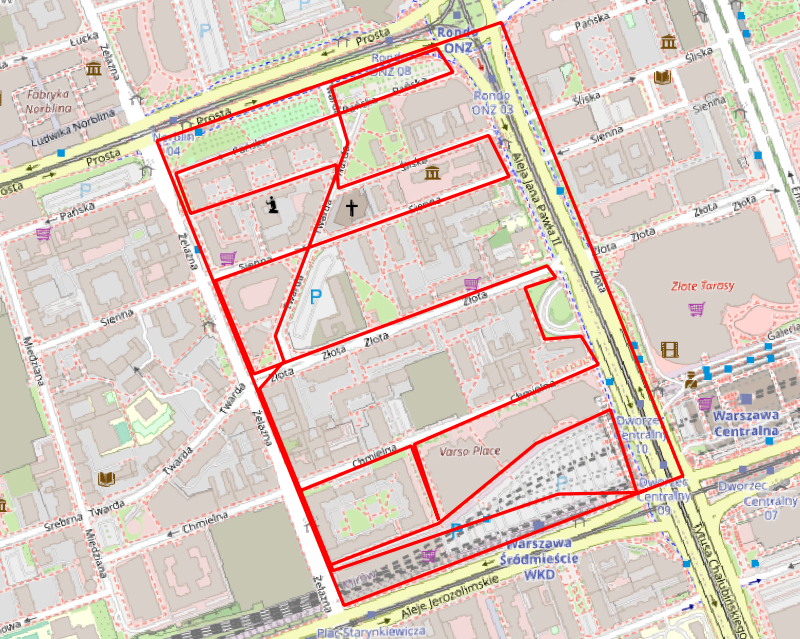
\includegraphics[width=1\linewidth]{route_p2}
			\caption{Planned route}
			\label{fig:a2}
		\end{subfigure}%
		\linebreak
		\begin{subfigure}{.90\textwidth}
			\centering
			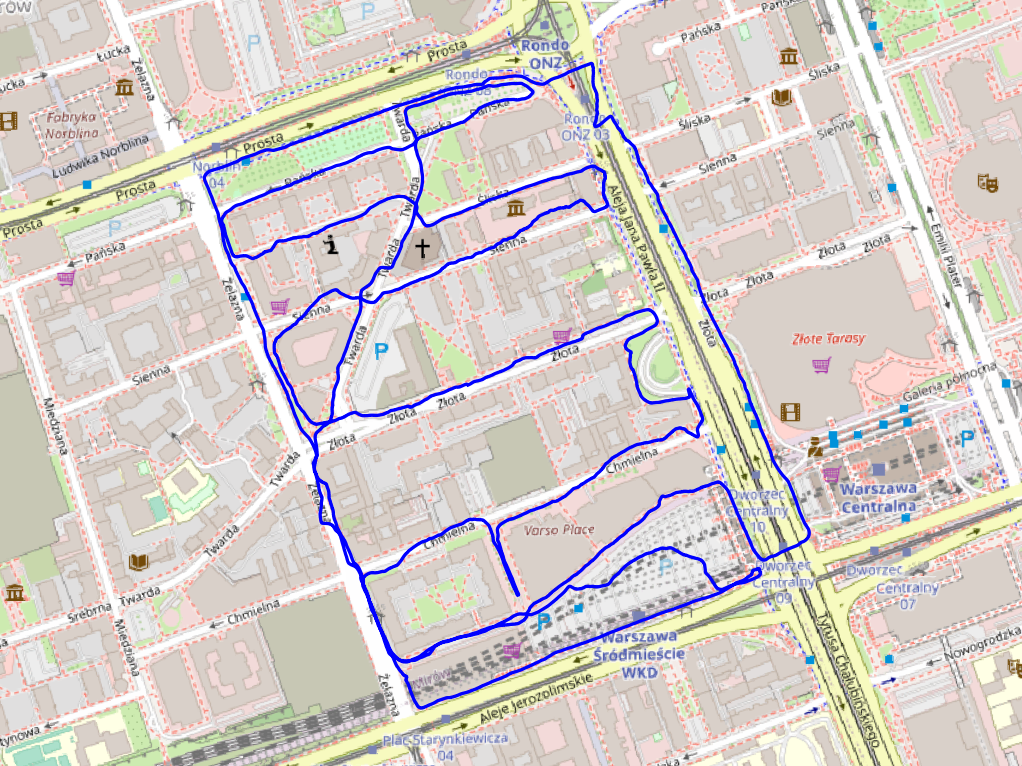
\includegraphics[width=1\linewidth]{route_c2}
			\caption{Covered route}
			\label{fig:b2}
		\end{subfigure}
		\caption{Planned and covered routes.}
		\label{fig:fig2}
	\end{figure}
	\item \textbf{19.09.2023} Next day on Tuesday area between Jerozolimskie avenue, Wspolna street, Chalubinskiego street and Marszalkowska street was scanned. Planned route measured 4,82km (Fig. 4a) and covered route 5,85km (Fig. 4b). Difference was caused again probably by localization problems in smartwach but also by my additional routes near Srodmiescie district office and Saint Barbara church.
	\begin{figure}[H]
		\centering
		\begin{subfigure}{.95\textwidth}
			\centering
			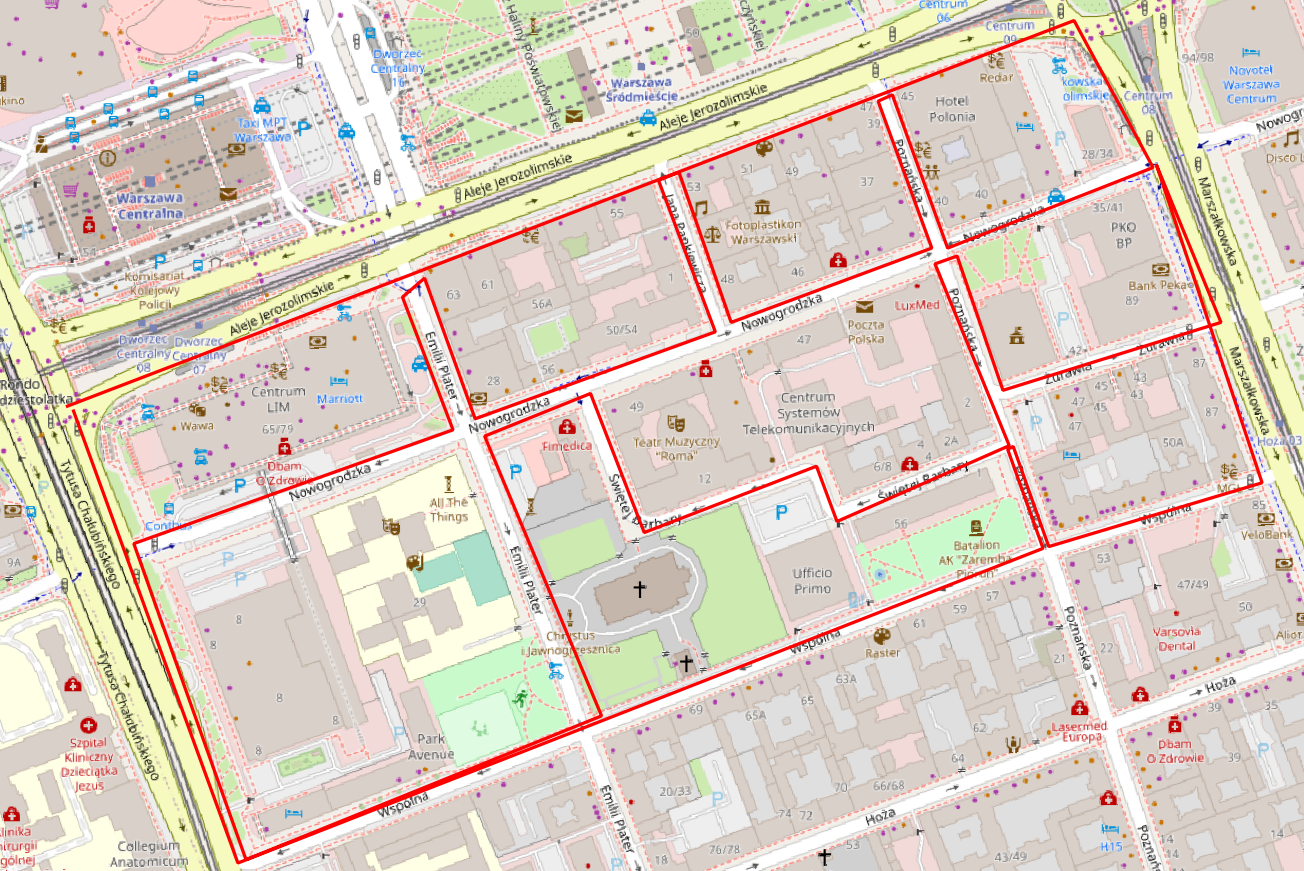
\includegraphics[width=1\linewidth]{route_p3}
			\caption{Planned route}
			\label{fig:a3}
		\end{subfigure}%
		\linebreak
		\begin{subfigure}{.95\textwidth}
			\centering
			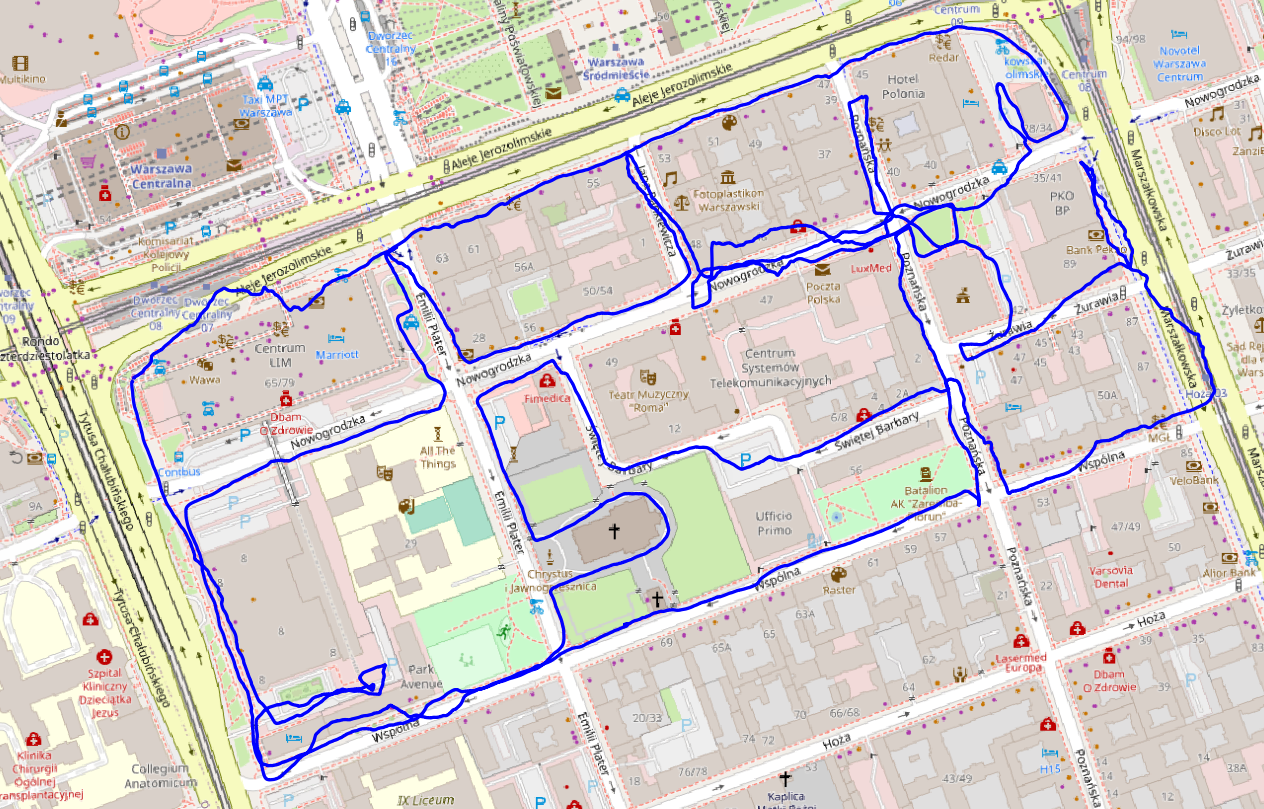
\includegraphics[width=1\linewidth]{route_c3}
			\caption{Covered route}
			\label{fig:b3}
		\end{subfigure}
		\caption{Planned and covered routes.}
		\label{fig:fig3}
	\end{figure}
	\pagebreak
	\item \textbf{20.09.2023} On this day scanning was performed near area from the day before, just a bit south, it included streets between Wspolna street, Koszykowa street, Chalubinskiego street and Marszalkowska street and also a fragment of Chalubinskiego street. Planned route was estimated to 5,06km (Fig. 5a) and ultimately reached similar distance: 4,99km (Fig.5b).
	\begin{figure}[H]
	\centering
	\begin{subfigure}{1\textwidth}
		\centering
		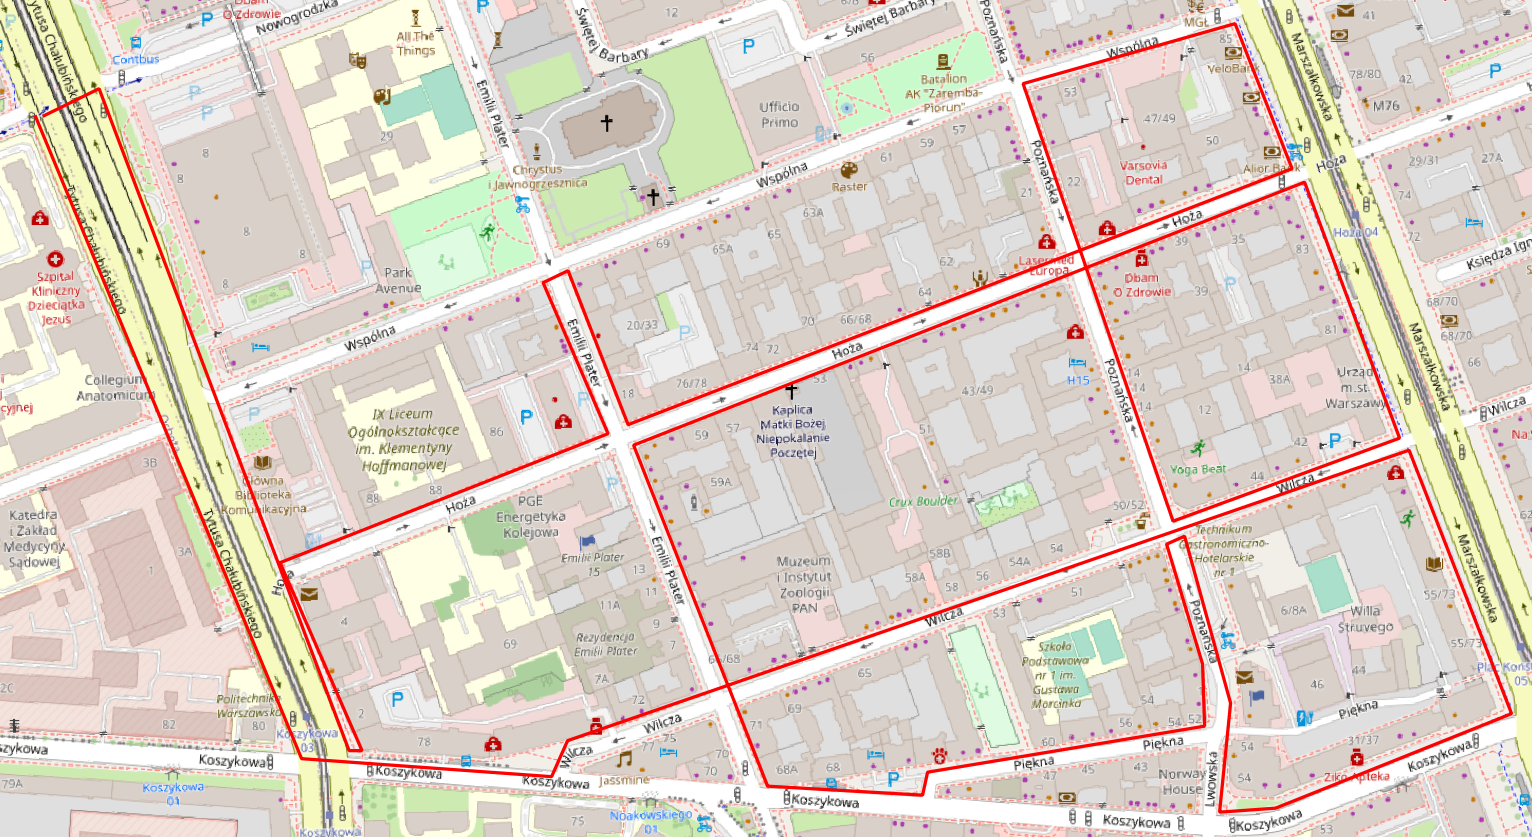
\includegraphics[width=1\linewidth]{route_p4}
		\caption{Planned route}
		\label{fig:a4}
	\end{subfigure}%
	\linebreak
	\begin{subfigure}{1\textwidth}
		\centering
		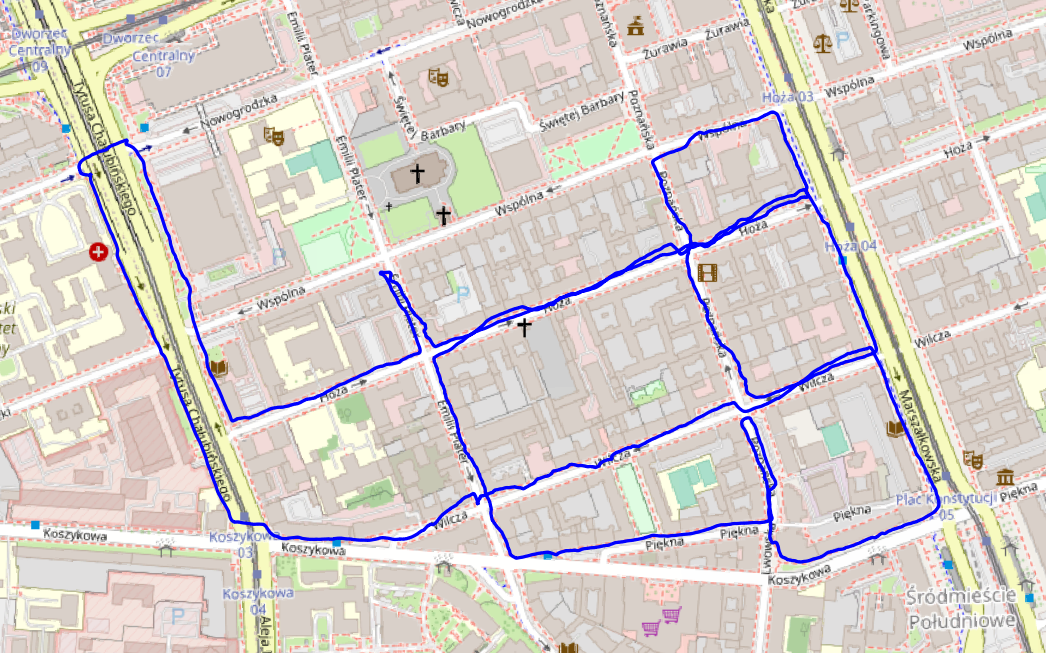
\includegraphics[width=1\linewidth]{route_c4}
		\caption{Covered route}
		\label{fig:b4}
	\end{subfigure}
	\caption{Planned and covered routes.}
	\label{fig:fig4}
\end{figure}
\pagebreak
\item \textbf{21.09.2023} That day scanning area encompassed Marszalkowska street, Constitution Square and surroundings around the main campus of Warsaw University of Technology. Planned route (Fig. 6a) was 5,78km and covered route (Fig. 6b), as well as most of the previous ones, exceeded this distance and summed up to  6,44km. 
\begin{figure}[H]
	\centering
	\begin{subfigure}{.80\textwidth}
		\centering
		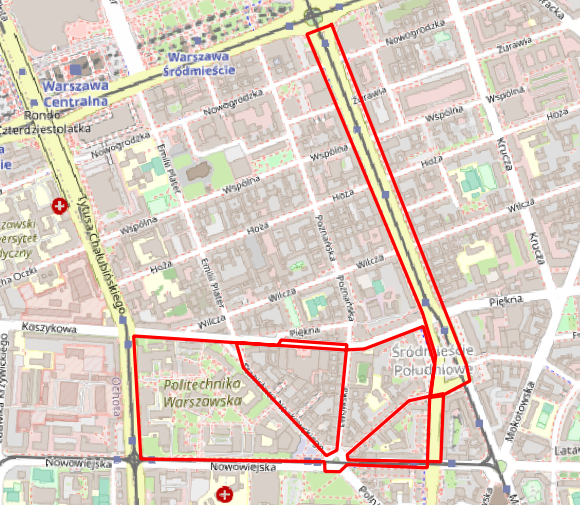
\includegraphics[width=1\linewidth]{route_p5}
		\caption{Planned route}
		\label{fig:a5}
	\end{subfigure}%
	\linebreak
	\begin{subfigure}{.80\textwidth}
		\centering
		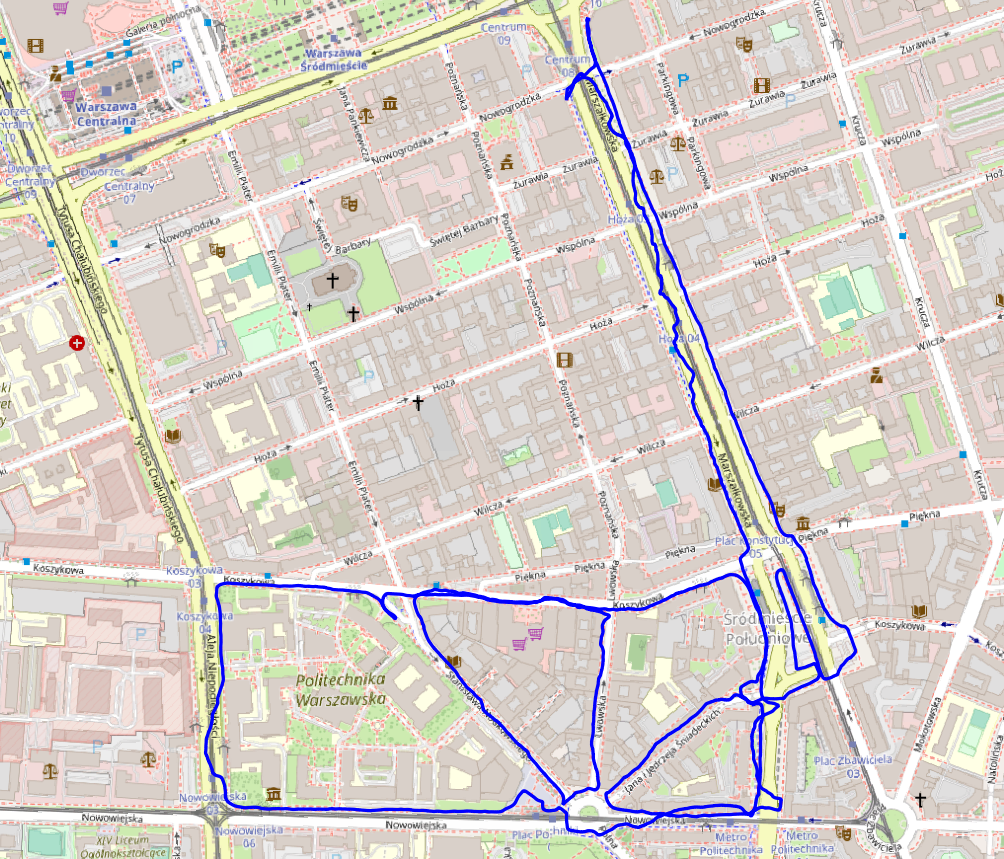
\includegraphics[width=1\linewidth]{route_c5}
		\caption{Covered route}
		\label{fig:b5}
	\end{subfigure}
	\caption{Planned and covered routes.}
	\label{fig:fig5}
\end{figure}
\item \textbf{22.09.2023} Scan was performed east of Marszalkowska street. Mostly it included Nowogrodzka street , Zurawia street, Wspolna street, Hoza street, Wilcza street and Krucza street. Planned route (Fig. 7a) was estimated to 5,65km, but as happened before, covered route (Fig. 7b) took longer and achieved 6,11km.
\begin{figure}[H]
	\centering
	\begin{subfigure}{.80\textwidth}
		\centering
		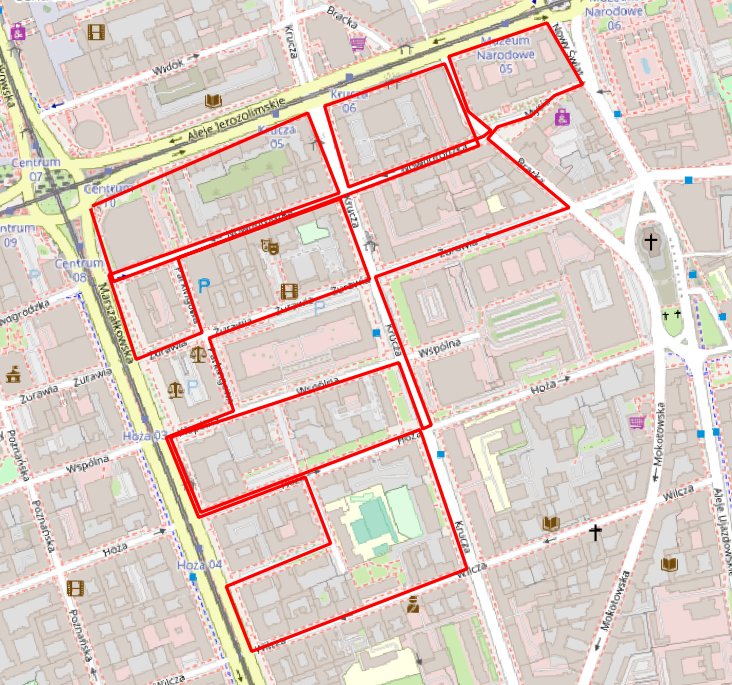
\includegraphics[width=1\linewidth]{route_p6}
		\caption{Planned route}
		\label{fig:a6}
	\end{subfigure}%
	\linebreak
	\begin{subfigure}{.80\textwidth}
		\centering
		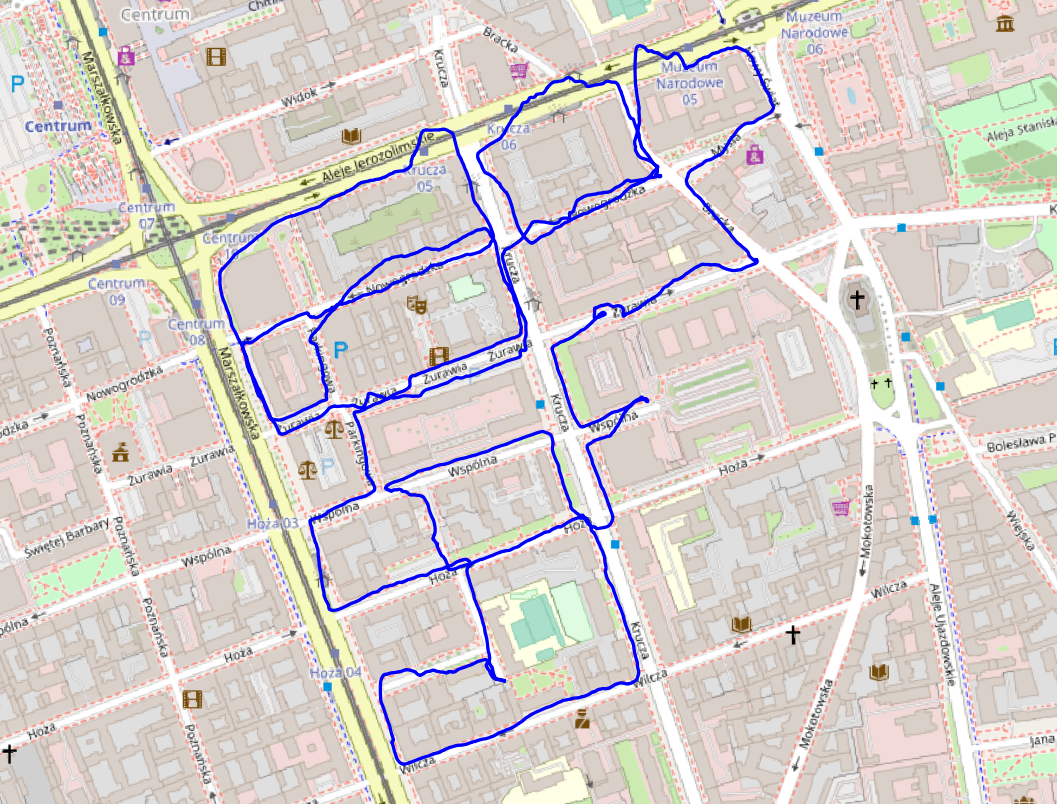
\includegraphics[width=1\linewidth]{route_c6}
		\caption{Covered route}
		\label{fig:b6}
	\end{subfigure}
	\caption{Planned and covered routes.}
	\label{fig:fig6}
\end{figure} 
\end{enumerate}

\section{Week 25-29 September 2023} 
\begin{enumerate}
	\item \textbf{25.09.2023} Scan was planned to be conducted in neighbourhood of Three Crosses Square. Total route was calculated to be 5,77km (Fig. 8a) but covered one (Fig. 8b) amounted to 7,38km due to my endeavors to fully cover Wiejska street and precisely scan the square.
	\begin{figure}[H]
		\centering
		\begin{subfigure}{.75\textwidth}
			\centering
			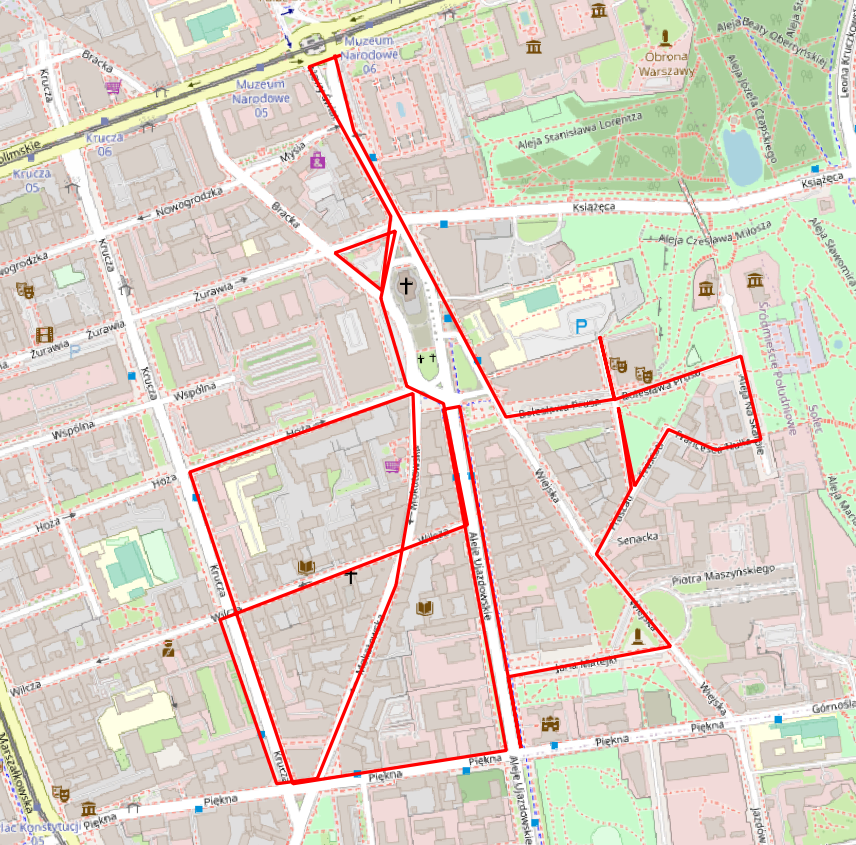
\includegraphics[width=1\linewidth]{route_p7}
			\caption{Planned route}
			\label{fig:a7}
		\end{subfigure}%
		\linebreak
		\begin{subfigure}{.75\textwidth}
			\centering
			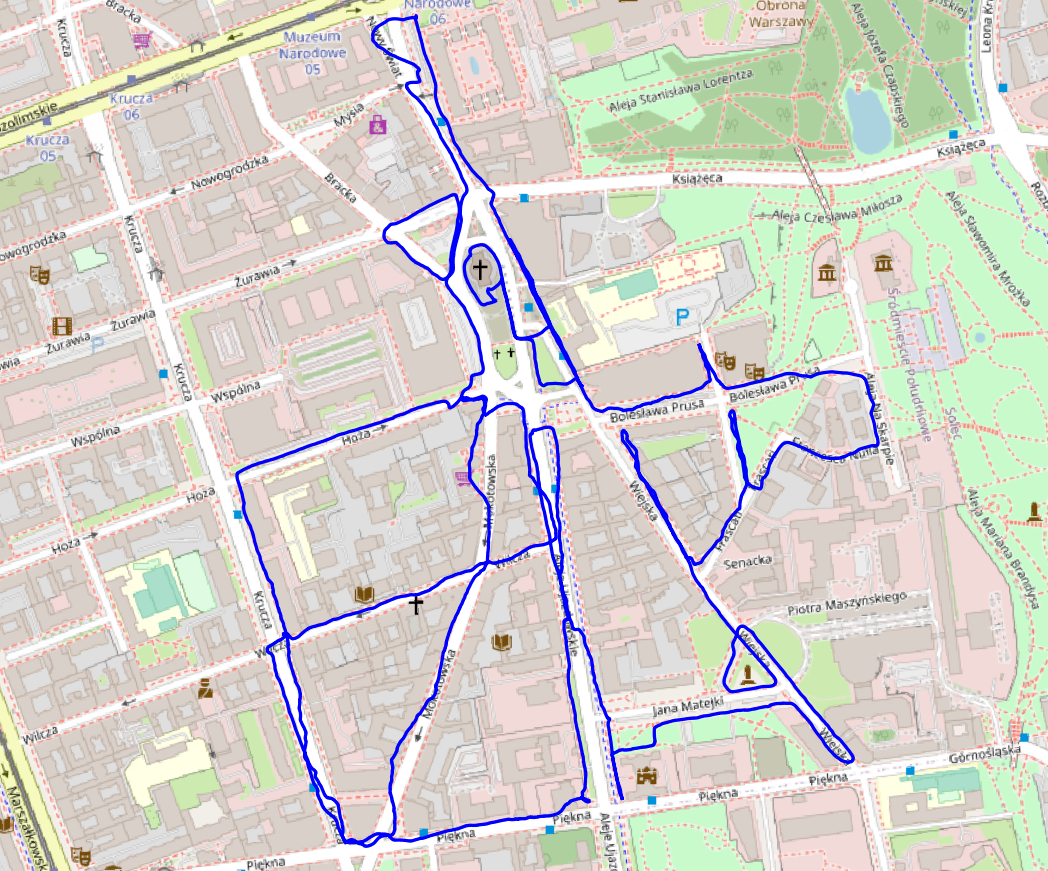
\includegraphics[width=1\linewidth]{route_c7}
			\caption{Covered route}
			\label{fig:b7}
		\end{subfigure}
		\caption{Planned and covered routes.}
		\label{fig:fig7}
	\end{figure} 
	\item \textbf{26.09.2023} Planned route (Fig. 9a) was estimated to 6,61km but covered route (Fig. 9b) reached 6,89km, mostly because of my efforts to scan Warsaw Insurgents Square as thoroughly as possible. It wasn't as easy as I had expected since during the time I was performing scans the square was undergoing reconstruction.
	\begin{figure}[H]
		\centering
		\begin{subfigure}{.83\textwidth}
			\centering
			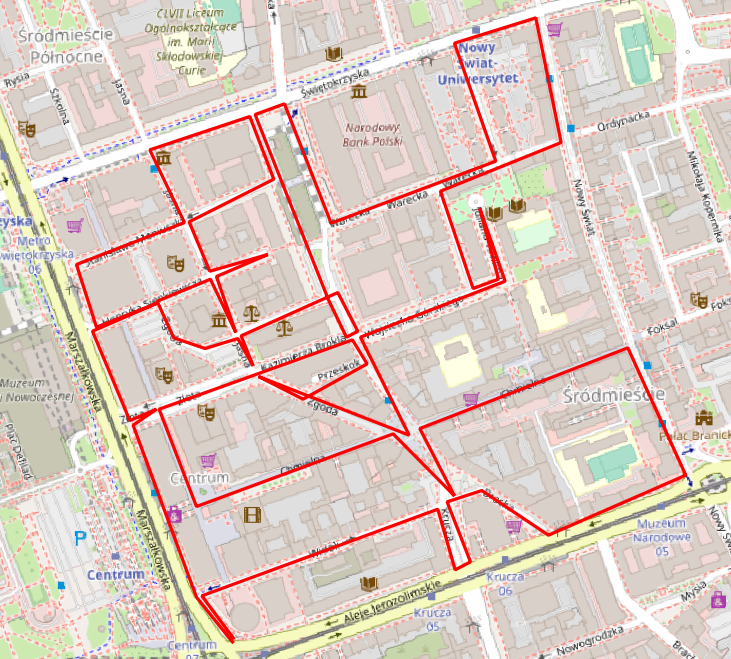
\includegraphics[width=1\linewidth]{route_p8}
			\caption{Planned route}
			\label{fig:a8}
		\end{subfigure}%
		\linebreak
		\begin{subfigure}{.83\textwidth}
			\centering
			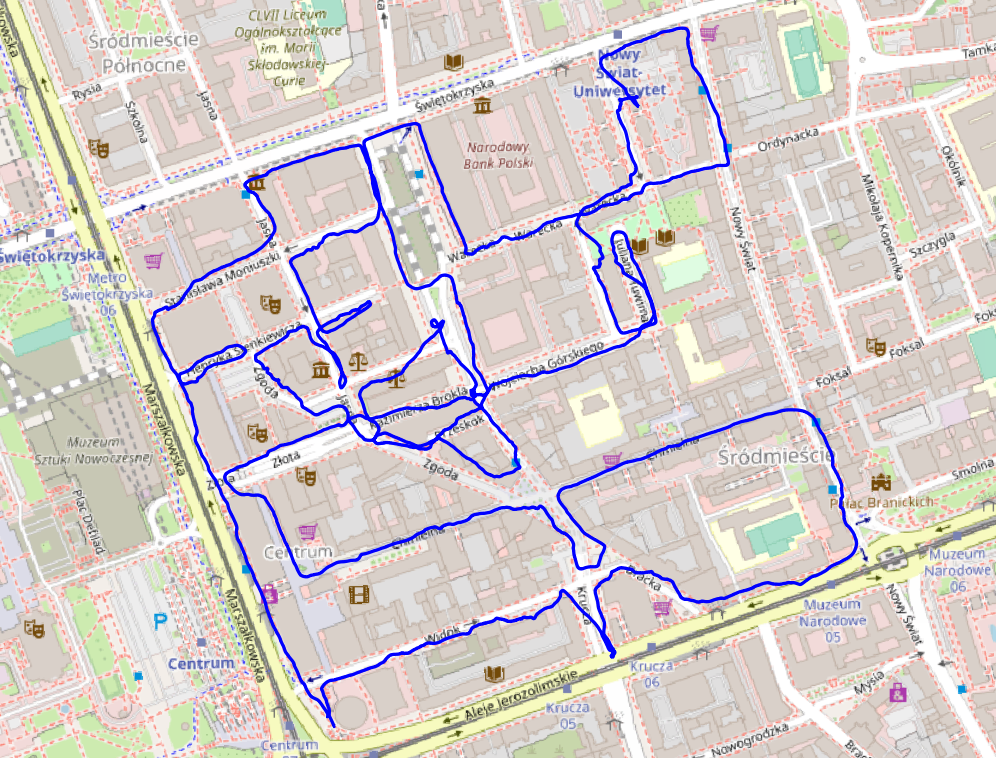
\includegraphics[width=1\linewidth]{route_c8}
			\caption{Covered route}
			\label{fig:b8}
		\end{subfigure}
		\caption{Planned and covered routes.}
		\label{fig:fig8}
	\end{figure} 
	\item \textbf{27.09.2023} Region to be scanned included streets between Swietokrzyska street, Krolewska street, Jana Pawla II avenue and Nowy Swiat street and route was planned to be 5,34km long (Fig. 10a). Longer covered route reached 5,82km (Fig. 10b) because of my mistake during scanning, I skipped one street and had to come back + forgot to turn smart watch on and started recording after a few minutes.
	\begin{figure}[H]
		\centering
		\begin{subfigure}{.93\textwidth}
			\centering
			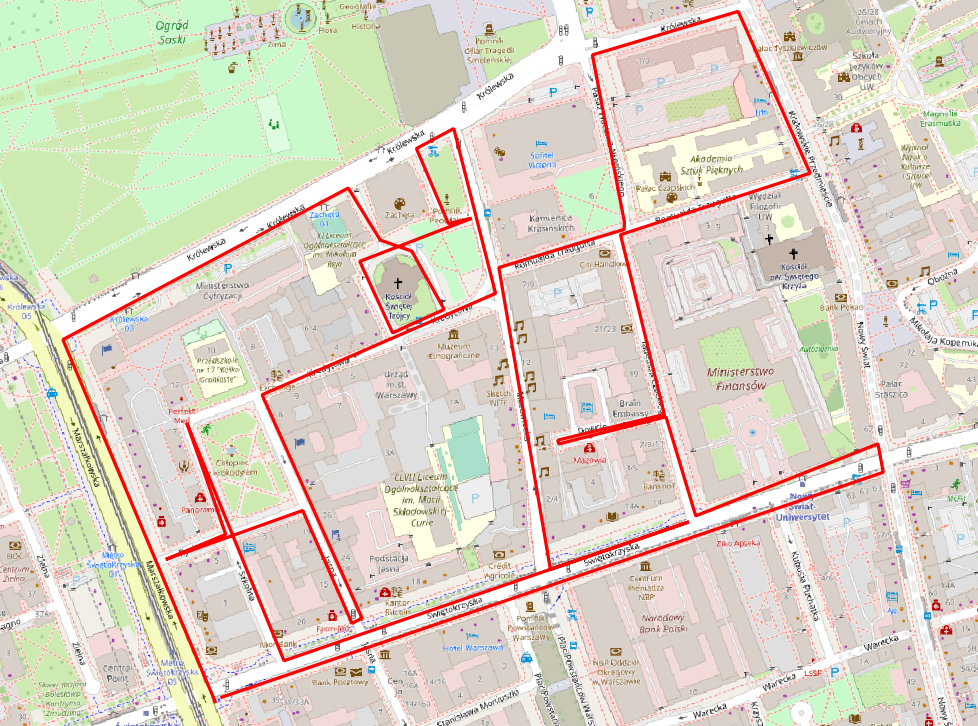
\includegraphics[width=1\linewidth]{route_p9}
			\caption{Planned route}
			\label{fig:a9}
		\end{subfigure}%
		\linebreak
		\begin{subfigure}{.93\textwidth}
			\centering
			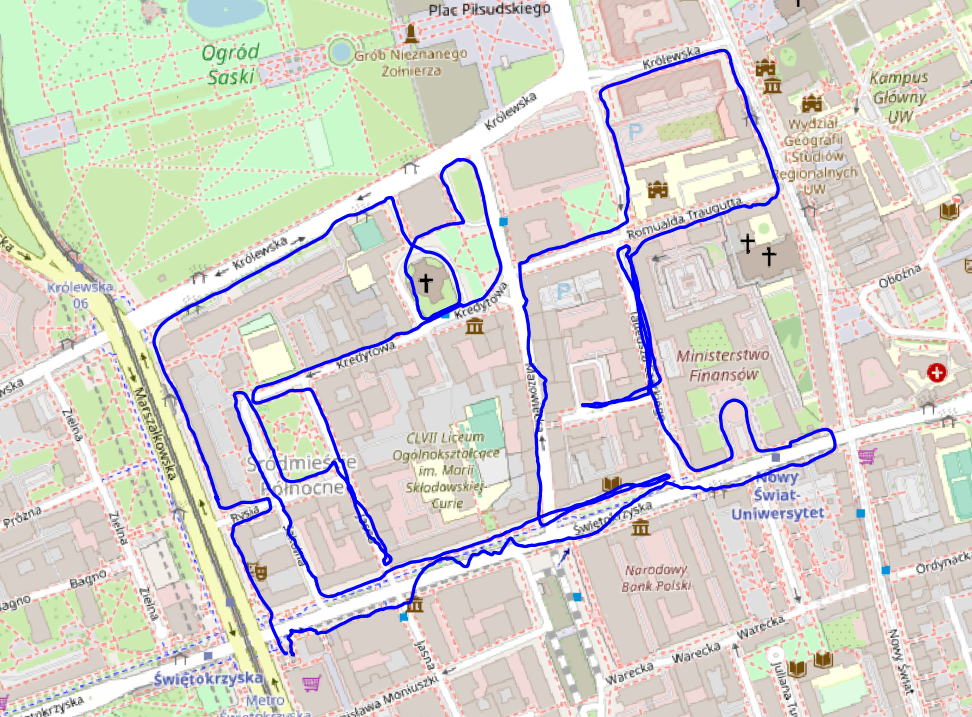
\includegraphics[width=1\linewidth]{route_c9}
			\caption{Covered route}
			\label{fig:b9}
		\end{subfigure}
		\caption{Planned and covered routes.}
		\label{fig:fig9}
	\end{figure} 
	\item \textbf{28.09.2023} Planned route was approximated to 6,46km (Fig. 11a), in neighbourhood of Mirowski square and streets north of Swietokrzyska street. Covered route 6,91km (Fig. 11b)
	\begin{figure}[H]
		\centering
		\begin{subfigure}{.90\textwidth}
			\centering
			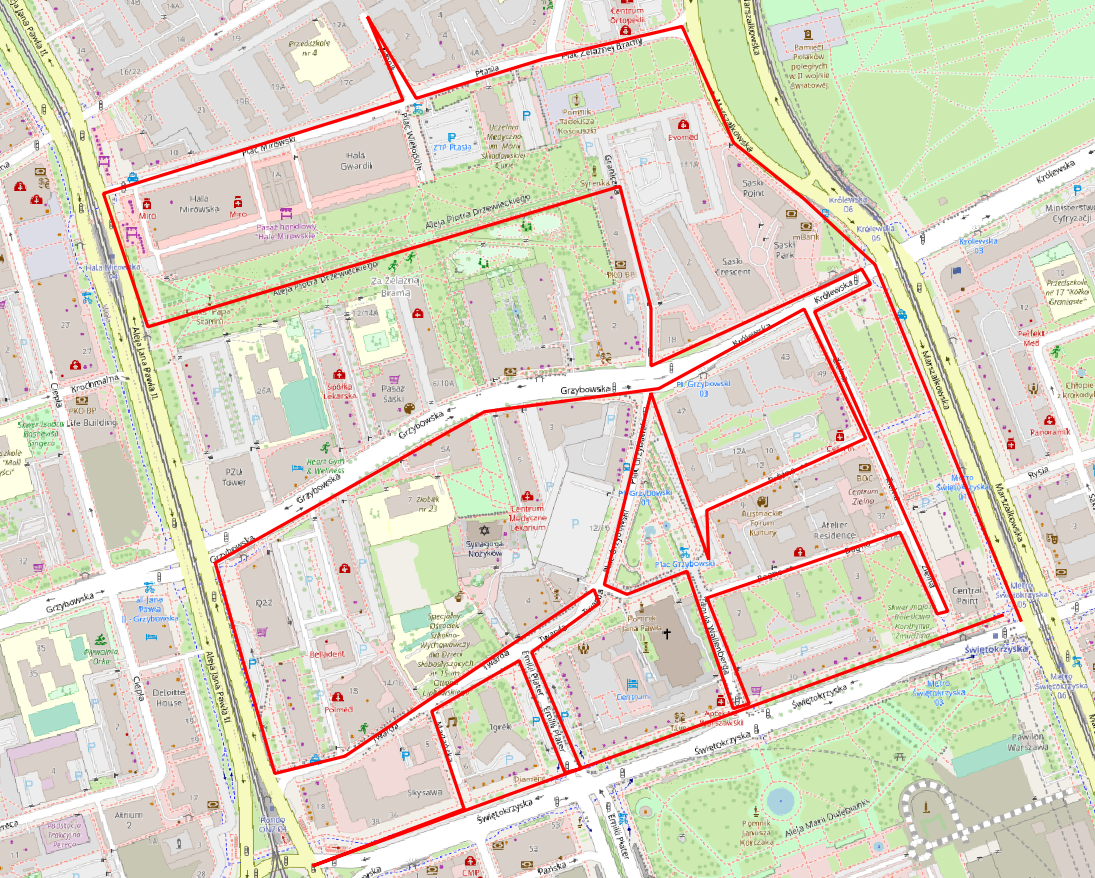
\includegraphics[width=1\linewidth]{route_p10}
			\caption{Planned route}
			\label{fig:a10}
		\end{subfigure}%
		\linebreak
		\begin{subfigure}{.90\textwidth}
			\centering
			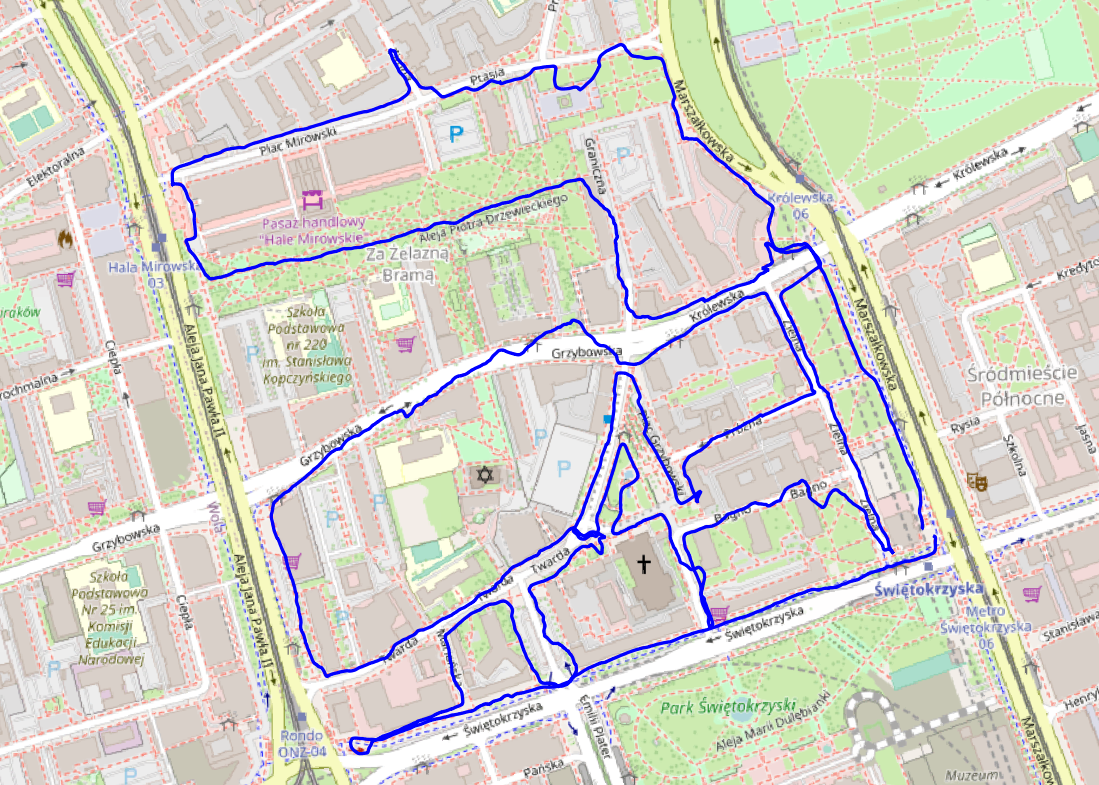
\includegraphics[width=1\linewidth]{route_c10}
			\caption{Covered route}
			\label{fig:b10}
		\end{subfigure}
		\caption{Planned and covered routes.}
		\label{fig:fig10}
	\end{figure} 
	\item \textbf{29.09.2023} This scan wasn't complicated nor long, it surrounded a scanning area for 2 October and was calculated to 4,62km (Fig. 12a). Covered route calculated to 4,85km (Fig. 12b)
	\begin{figure}[H]
		\centering
		\begin{subfigure}{.88\textwidth}
			\centering
			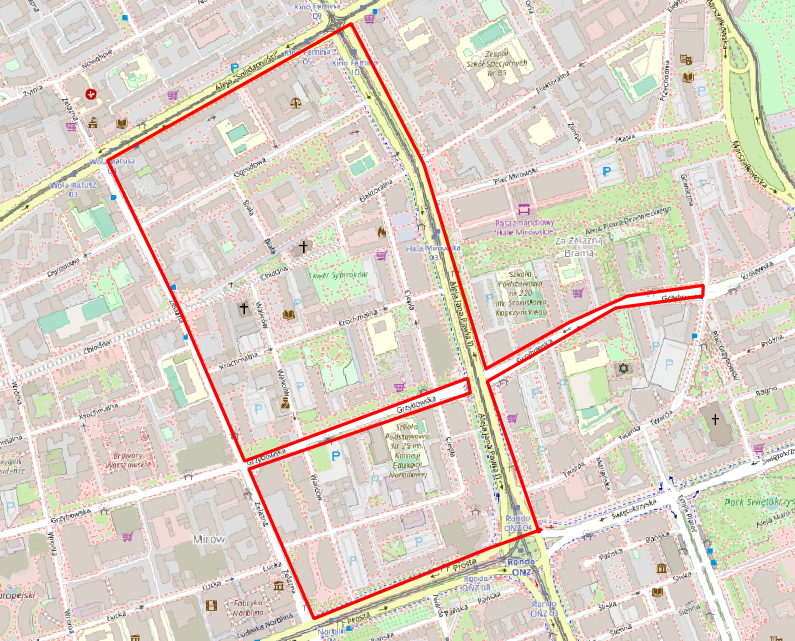
\includegraphics[width=1\linewidth]{route_p11}
			\caption{Planned route}
			\label{fig:a11}
		\end{subfigure}%
		\linebreak
		\begin{subfigure}{.88\textwidth}
			\centering
			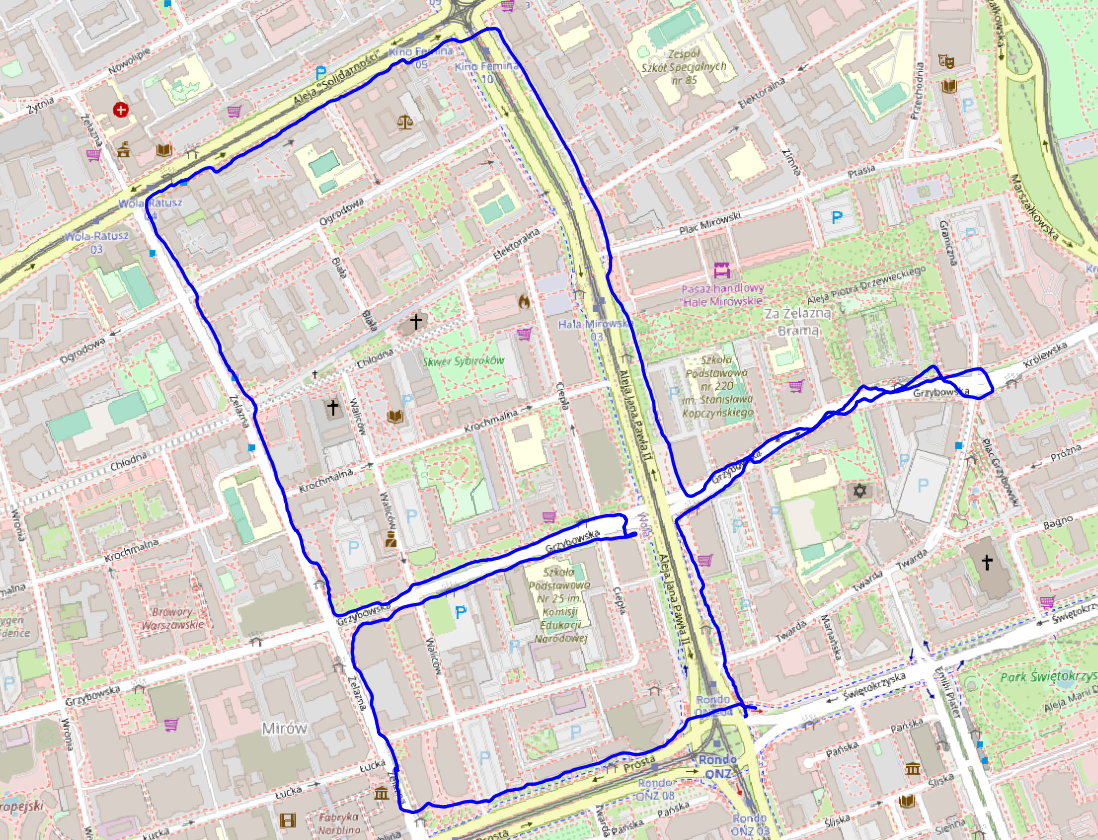
\includegraphics[width=1\linewidth]{route_c11}
			\caption{Covered route}
			\label{fig:b11}
		\end{subfigure}
		\caption{Planned and covered routes.}
		\label{fig:fig11}
	\end{figure} 
\end{enumerate}

\section{Week 2-6 October 2023}
\begin{enumerate}
	\item \textbf{02.10.2023} Scanned streets between "Solidarnosci" avenue, Zelazna street, Jana Pawla II avenue and Prosta street. Route according to plan supposed to have 6,23km (Fig. 13a) and as happened earlier covered route was a little bit longer, because it had 6,65km (Fig. 13b)
	\begin{figure}[H]
		\centering
		\begin{subfigure}{.77\textwidth}
			\centering
			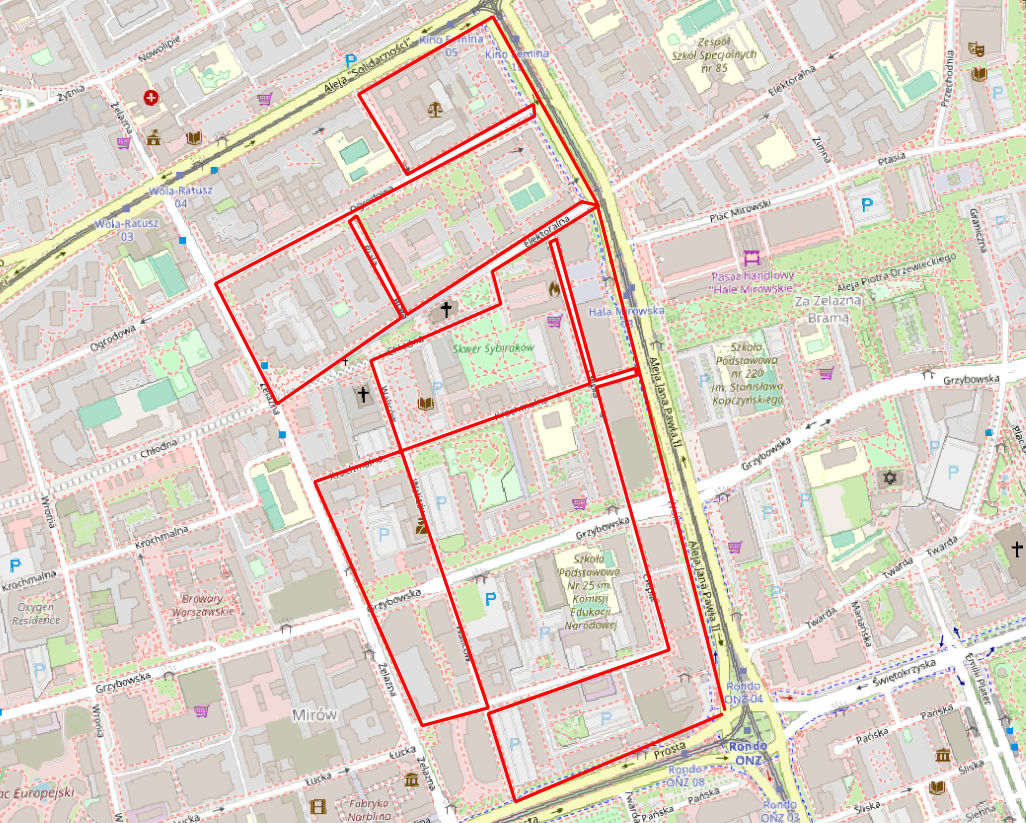
\includegraphics[width=1\linewidth]{route_p12}
			\caption{Planned route}
			\label{fig:a12}
		\end{subfigure}%
		\linebreak
		\begin{subfigure}{.77\textwidth}
			\centering
			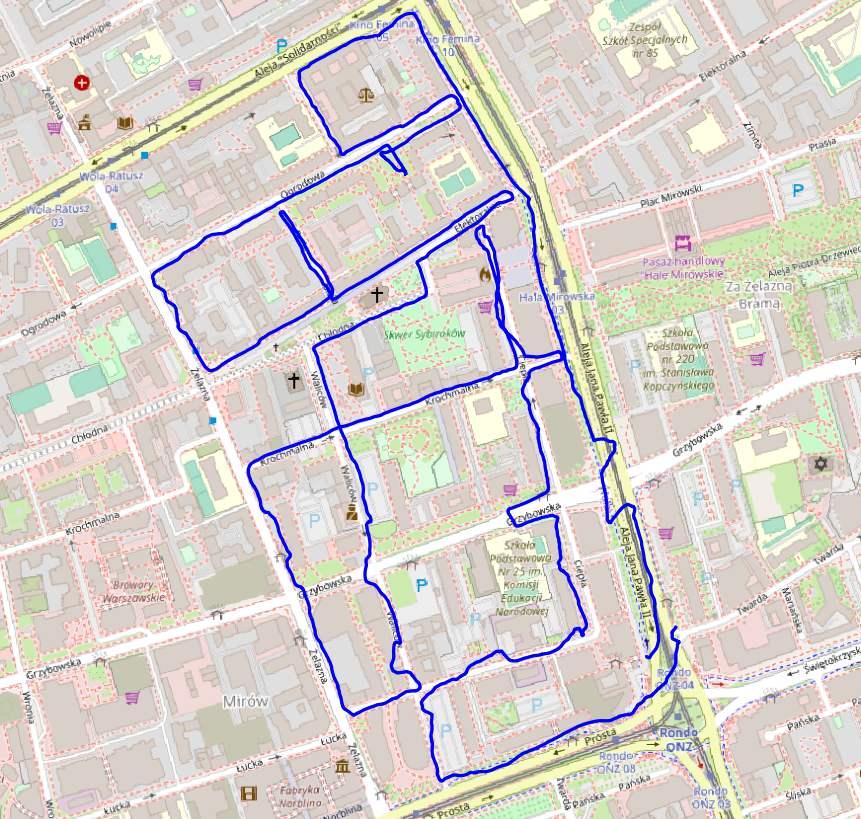
\includegraphics[width=1\linewidth]{route_c12}
			\caption{Covered route}
			\label{fig:b12}
		\end{subfigure}
		\caption{Planned and covered routes.}
		\label{fig:fig12}
	\end{figure} 
	\item \textbf{03.10.2023} Route was planned to thoroughly scan Jerozolimskie avenue and create some kind of connector between different point clouds. Planned length was equal to 4,72km (Fig. 14a), but covered length was longer - 5,45km (Fig. 14b). This was caused by localizations of pedestrian crossings that weren't as straight as was planned and some detours were needed.
	\begin{figure}[H]
		\centering
		\begin{subfigure}{.77\textwidth}
			\centering
			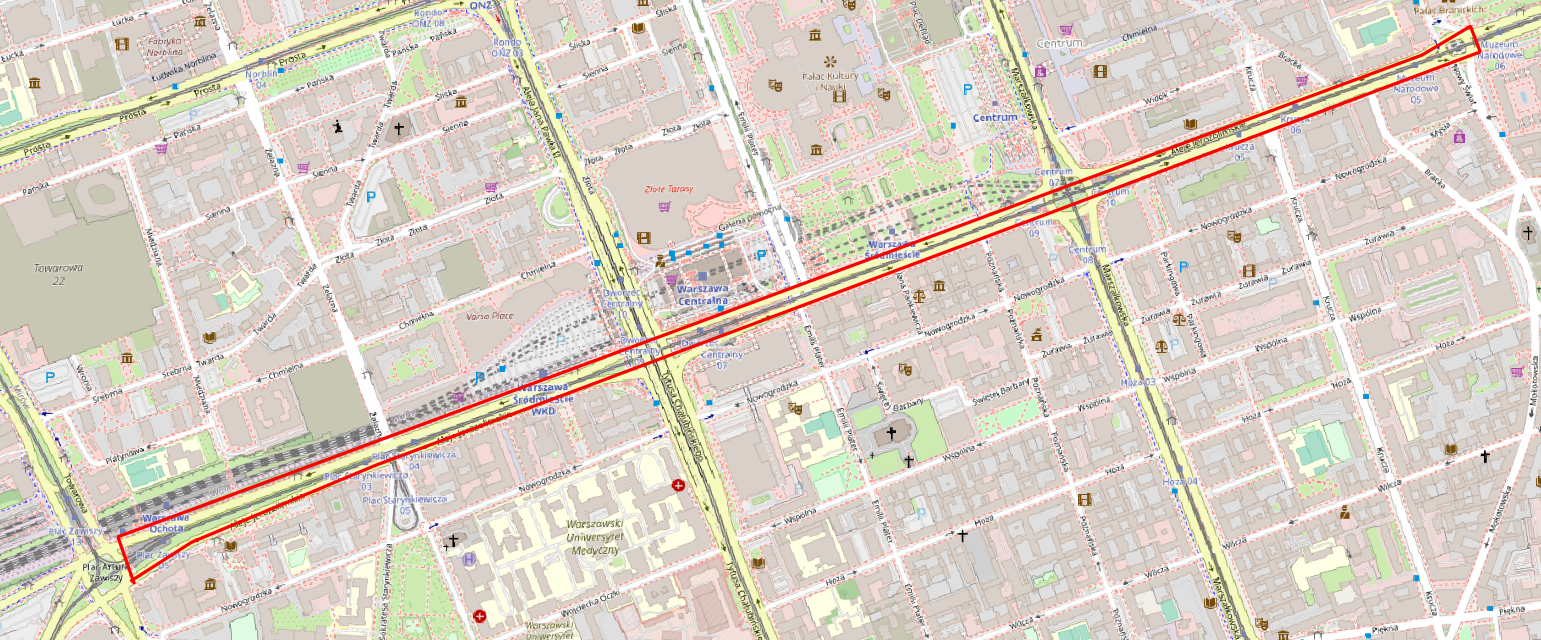
\includegraphics[width=1\linewidth]{route_p13}
			\caption{Planned route}
			\label{fig:a13}
		\end{subfigure}%
		\linebreak
		\begin{subfigure}{.77\textwidth}
			\centering
			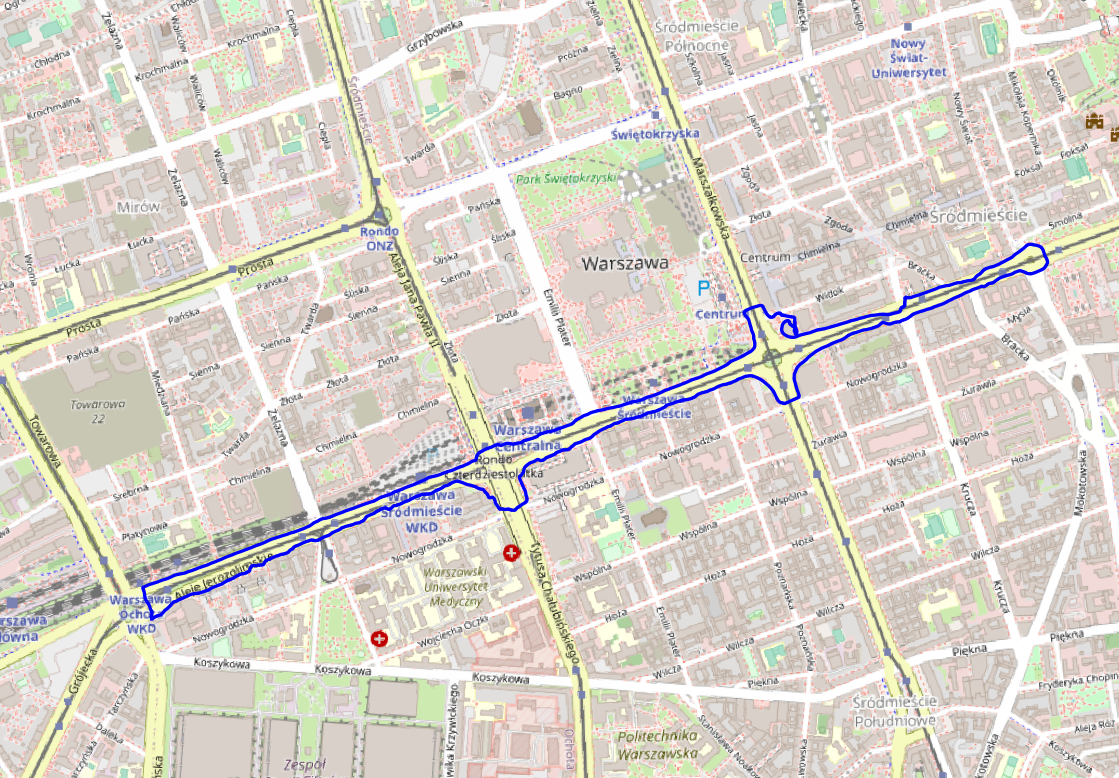
\includegraphics[width=1\linewidth]{route_c13}
			\caption{Covered route}
			\label{fig:b13}
		\end{subfigure}
		\caption{Planned and covered routes.}
		\label{fig:fig13}
	\end{figure} 
	\item \textbf{04.10.2023} Streets covered by the scan were all located between Prosta street, Towarowa street, Jerozolimskie avenue and Zelazna street. Planned length of the scanning route was estimated to 5,09km (Fig. 15a) and covered route reached 5,58km (Fig. 15b), probably because of additional scanning path near one of the skyscrapers. The path can be seen at the bottom part of Fig. 15b as the difference from Fig. 15a.
	\begin{figure}[H]
		\centering
		\begin{subfigure}{.77\textwidth}
			\centering
			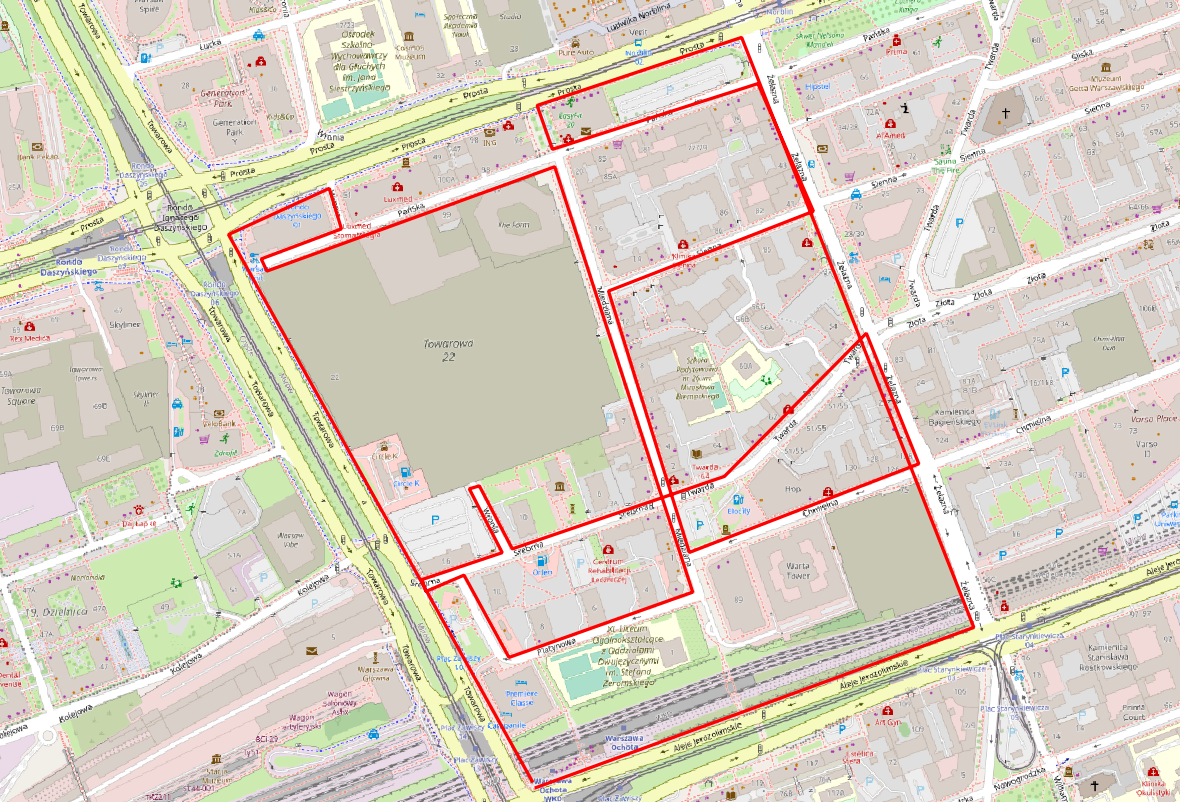
\includegraphics[width=1\linewidth]{route_p14}
			\caption{Planned route}
			\label{fig:a14}
		\end{subfigure}%
		\linebreak
		\begin{subfigure}{.77\textwidth}
			\centering
			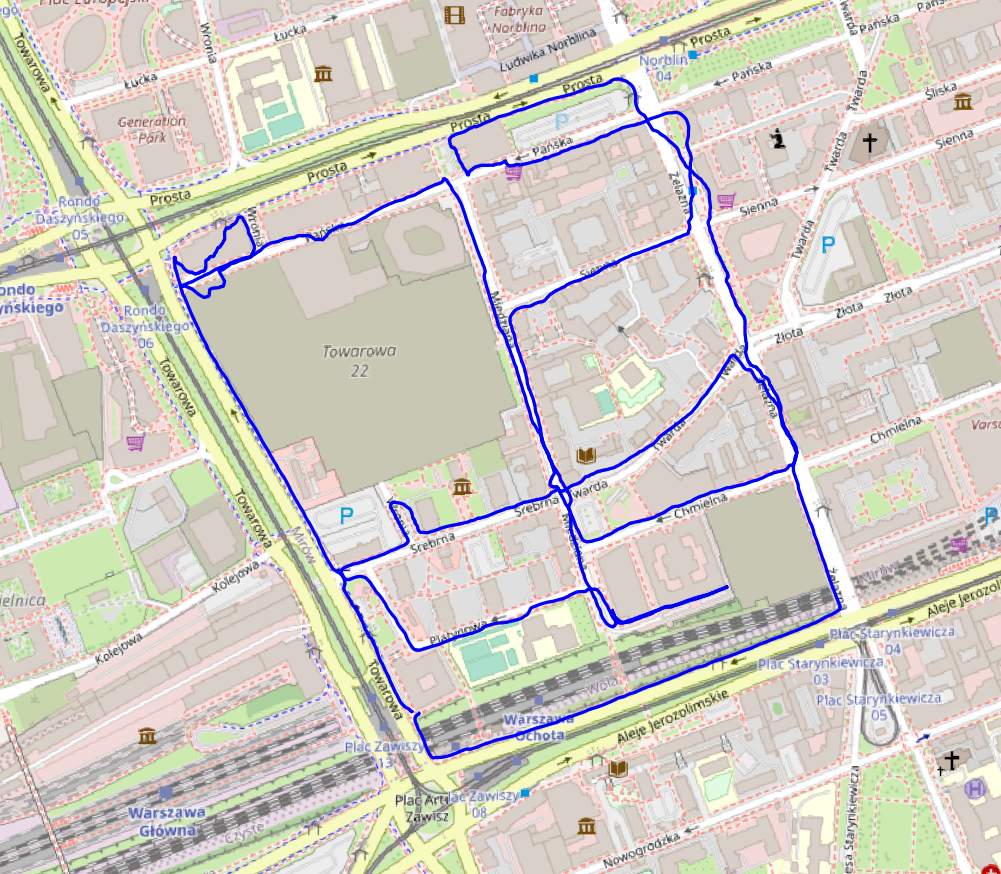
\includegraphics[width=1\linewidth]{route_c14}
			\caption{Covered route}
			\label{fig:b14}
		\end{subfigure}
		\caption{Planned and covered routes.}
		\label{fig:fig14}
	\end{figure} 
	\item \textbf{05.10.2023} Scan was performed north of the previous one, on the opposite site of Prosta street. Planned route length equals 5,07km (Fig. 16a) and covered one equals 6,3km. Higher covered length is partly caused due to my mistake in the beginning of the scan - i chose wrong path as seen at the bottom of Fig. 16b as it has additional line in comparison to Fig. 16b. The main reason why covered route is longer is that I scanned Krochmalna street (seen at the middle of Fig. 16b) that wasn't included in the planned routes, since it wasn't added to the database BDOT10k yet, hence the difference. 
	\begin{figure}[H]
		\centering
		\begin{subfigure}{.77\textwidth}
			\centering
			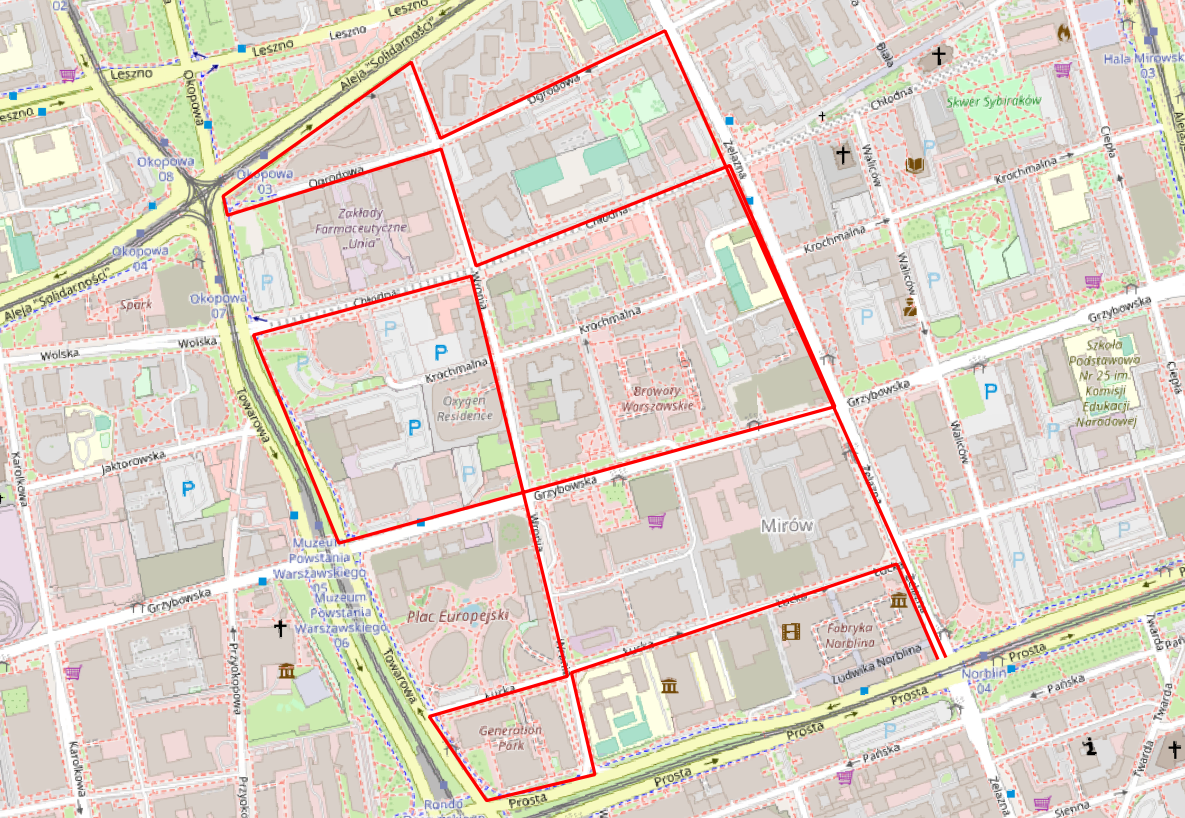
\includegraphics[width=1\linewidth]{route_p15}
			\caption{Planned route}
			\label{fig:a15}
		\end{subfigure}%
		\linebreak
		\begin{subfigure}{.77\textwidth}
			\centering
			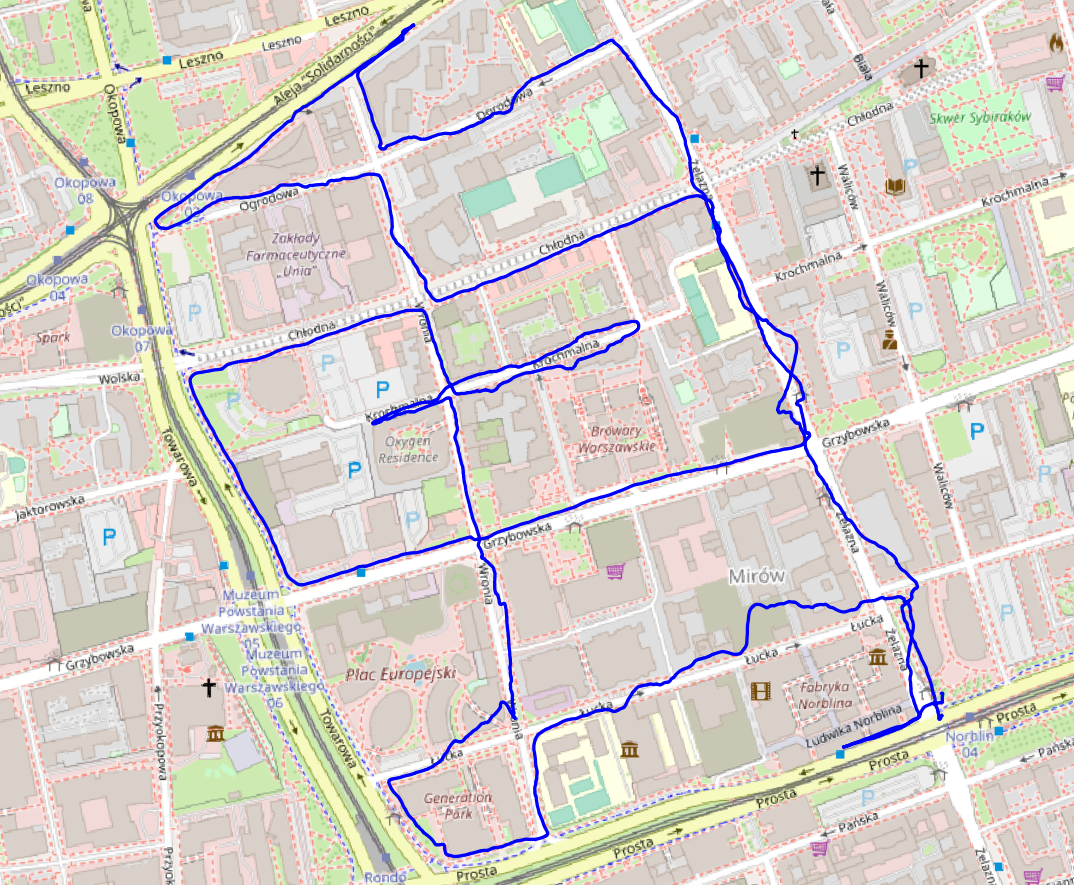
\includegraphics[width=1\linewidth]{route_c15}
			\caption{Covered route}
			\label{fig:b15}
		\end{subfigure}
		\caption{Planned and covered routes.}
		\label{fig:fig15}
	\end{figure} 
\end{enumerate}

\section{Week 9-13 October 2023}

\section{Week 16-20 October 2023}

\section{Week 23-27 October 2023}

\section{Week 30-31 October 1-3 November 2023}

\end{document}
